\chapter{代码生成}

\section{类型检查}

\subsection{类型检查(Type Checking)}

经过词法分析后,词法分析器将token流传递给语法分析器,语法分析器将生成一个语法树。当源代码转换为语法树时,类型检查器起着至关重要的作用。通过查看语法树,您可以判断每种数据类型是否正在处理正确的变量。\\

类型检查主要是为了判断变量或者参数的实际类型和声明的类型是否匹配。类型检查可以及早地发现类型不匹配的问题,不要等到执行的时候才发现问题。提前发现问题可以降低成本。\\

每种语言都有自己的语言类型规则集,编译器必须检查源程序是否遵循语言的句法和语义约定。它限制程序员在某些情况下可以使用的类型并将类型分配给值。\\

编译器需要检查对象的类型并在违反的情况下报告类型错误,并纠正不正确的类型。\\

如果要由编译器自动完成从一种类型到另一种类型的转换,则称为隐式转换(implicit conversion)。例如整数可以转换为实数,而实数不能转换为整数。而需要由程序员明确指定的类型转换被称为显示类型转换(explicit conversion),也称为强制类型转换。\\

\subsection{静态类型检查(Staic Type Checking)}

静态类型检查发生在编译期间,它在编译时检查变量的类型,这意味着变量的类型在编译时是已知的。\\

静态类型检查包括:

\begin{itemize}
    \item 类型检查:如果将运算符应用于不匹配的操作数,编译器需要报告错误。例如将一个数组变量和函数相加。

    \item 控制流检查:一些能够导致离开某个控制结构的语句,应该存在能够被转移到的位置。例如C中的break语句会导致离开离它最近的while、for或switch结构,如果这样的结构不存在,则会发生错误。

    \item 唯一性检查:在某些情况下,对象只可以定义一次。例如Pascal中标识符必须唯一声明,case语句中的标签必须是不同的。

    \item 名称检查:有时同一个名称可能会出现两次或多次。例如Ada中循环的名称可能出现在结构的开头和结尾。编译器必须检查两个地方是否使用了相同的名称。
\end{itemize}

静态类型检查能够有效发现语法错误和错误的名称,例如额外的标点符号或写错了预定义的名称。对于函数而言,可以检查函数参数的类型和数量是否匹配。\\

\subsection{动态类型检查(Dynamic Type Checking)}

动态类型检查发生在运行时,即当涉及到具体的数据值时才进行类型检查。动态类型检查提供了更宽松、灵活的程序设计环境,在交互式语言中十分有用。\\

动态类型语言一般是脚本语言,如Perl、Ruby、Python、PHP、JavaScript等,可以更快地编写代码,不必每次都指定类型。\\

但是动态类型检查有着一些缺陷。首先它增加了程序的运行时间,影响了效率。同时动态类型检查错误发现太晚,不能防止运行时产生出错。

\newpage

\section{运行时环境}

\subsection{存储分配}

编译器在工作过程中,必须为源程序中出现的一些数据对象分配运行时的存储空间。对于那些在编译时刻就可以确定大小的数据对象,可以在编译时刻就为它们分配存储空间,这样的分配策略称为静态存储分配。\\

如果不能在编译时完全确定数据对象的大小,就要采用动态存储分配的策略。即在编译时仅产生各种必要的信息,而在运行时刻,再动态地分配数据对象的存储空间。这包括了栈式存储分配和堆式存储分配。\\

\begin{figure}[H]
    \centering
    \begin{tikzpicture}[scale=0.7]
        \draw[-] (0,0) -- (0,10) -- (5,10) -- (5,0) -- (0,0);
        \draw[-] (0,2) -- (5,2);
        \draw[-] (0,4) -- (5,4);
        \draw[-] (0,6) -- (5,6);
        \draw[-] (0,8) -- (5,8);

        \draw[-] (2.5,9) node {静态代码区};
        \draw[-] (2.5,7) node {静态数据区};
        \draw[-] (2.5,5) node {栈(Stack)};
        \draw[-] (2.5,1) node {堆(Heap)};

        \draw[->] (2.5,4) -- (2.5,3.5);
        \draw[->] (2.5,2) -- (2.5,2.5);
    \end{tikzpicture}
    \caption{内存管理}
\end{figure}

编译程序生成的代码大小通常是固定的,一般存放在代码区。目标程序运行过程中,需要创建和访问的数据对象存放在数据区。\\

栈区由编译器自动分配和释放,存放函数的参数值、局部变量的值等。\\

在编译时刻不能确定大小的对象将被分配在堆区,堆区的空间一般由程序员分配和释放。若程序员不释放,程序结束后被操作系统改回收。\\

\subsection{活动记录(Activation Record)}

编译器通常以过程(或函数、方法)为单位分配存储空间,过程体的每次执行称为该过程的一个活动,过程每执行一次,就为它分配一块连续存储区,用来管理过程一次执行所需的信息。\\

活动记录中包括:

\begin{itemize}
    \item 实参
    \item 返回值
    \item 控制链:指向调用者的活动记录
    \item 访问链:用来访问存放于其它活动记录中的非局部数据
    \item 保存的机器状态
    \item 局部数据
    \item 临时变量
\end{itemize}

过程的存储以栈的形式进行管理,当一个过程被调用时,该过程的活动记录被压入栈;当过程结束时,该活动记录被弹出栈。\\

过程调用和过程返回都需要执行一些代码来管理活动记录栈,保存或恢复机器状态等。其中,调用过程时需要为一个活动记录在栈中分配空间,并在此记录的字段中填写信息。过程返回需要恢复机器状态,使得在调用结束之后继续执行。

\newpage

\section{中间代码生成}

\subsection{中间代码生成(Intermediate Code Generation)}

源代码可以直接翻译成目标机器码,但是为什么要将其先翻译成中间代码,再翻译成目标代码呢?\\

如果没有中间代码,那么每种语言都需要为每种目标机器都设计一个编译器。如果使用中间代码表示(intermediate representation),将会使需要设计的编译器少得多。\\

\begin{figure}[H]
    \centering
    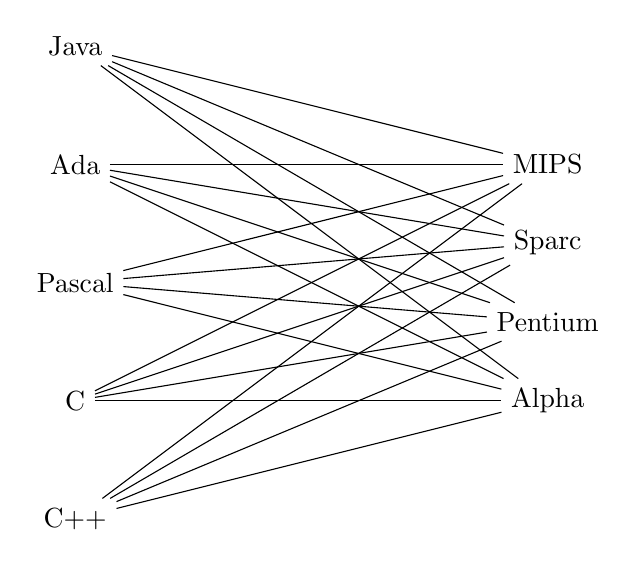
\begin{tikzpicture}
        \node (Java) at (-3,3) {Java};
        \node (Ada) at (-3,1.5) {Ada};
        \node (Pascal) at (-3,0) {Pascal};
        \node (C) at (-3,-1.5) {C};
        \node (C++) at (-3,-3) {C++};

        \node (Sparc) at (3,0.5) {Sparc};
        \node (MIPS) at (3,1.5) {MIPS};
        \node (Pentium) at (3,-0.5) {Pentium};
        \node (Alpha) at (3,-1.5) {Alpha};

        \draw[-] (Java) -- (Sparc);
        \draw[-] (Java) -- (MIPS);
        \draw[-] (Java) -- (Pentium);
        \draw[-] (Java) -- (Alpha);
        \draw[-] (Ada) -- (Sparc);
        \draw[-] (Ada) -- (MIPS);
        \draw[-] (Ada) -- (Pentium);
        \draw[-] (Ada) -- (Alpha);
        \draw[-] (Pascal) -- (Sparc);
        \draw[-] (Pascal) -- (MIPS);
        \draw[-] (Pascal) -- (Pentium);
        \draw[-] (Pascal) -- (Alpha);
        \draw[-] (C) -- (Sparc);
        \draw[-] (C) -- (MIPS);
        \draw[-] (C) -- (Pentium);
        \draw[-] (C) -- (Alpha);
        \draw[-] (C++) -- (Sparc);
        \draw[-] (C++) -- (MIPS);
        \draw[-] (C++) -- (Pentium);
        \draw[-] (C++) -- (Alpha);
    \end{tikzpicture}

    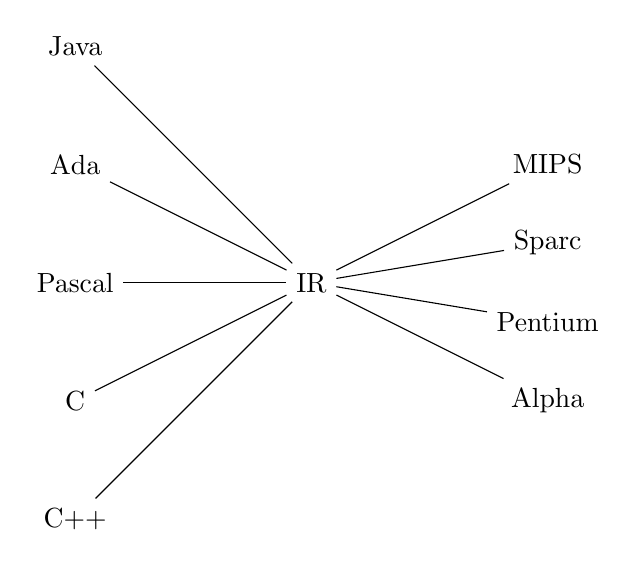
\begin{tikzpicture}
        \node (Java) at (-3,3) {Java};
        \node (Ada) at (-3,1.5) {Ada};
        \node (Pascal) at (-3,0) {Pascal};
        \node (C) at (-3,-1.5) {C};
        \node (C++) at (-3,-3) {C++};

        \node (IR) at (0,0) {IR};

        \node (Sparc) at (3,0.5) {Sparc};
        \node (MIPS) at (3,1.5) {MIPS};
        \node (Pentium) at (3,-0.5) {Pentium};
        \node (Alpha) at (3,-1.5) {Alpha};

        \draw[-] (Java) -- (IR);
        \draw[-] (Ada) -- (IR);
        \draw[-] (Pascal) -- (IR);
        \draw[-] (C) -- (IR);
        \draw[-] (C++) -- (IR);
        \draw[-] (IR) -- (Sparc);
        \draw[-] (IR) -- (MIPS);
        \draw[-] (IR) -- (Pentium);
        \draw[-] (IR) -- (Alpha);
    \end{tikzpicture}
    \caption{中间代码}
\end{figure}

中间代码不依赖目标机的结构,中间语言与具体机器特性无关,一种中间语言可以为生成多种不同型号的目标机的目标代码服务。因此,对于中间语言,要求其不但与机器无关,而且有利于代码生成。\\

\subsection{三地址码(Three Address Code)}

三地址码是一种易于生成且易于转换为机器码的中间代码,它最多使用三个地址和一个运算符来表示一个表达式。\\

\subsubsection{算术表达式}

例如$ 2 * a + (b - 3) $用三地址码表示为:

\vspace{-0.5cm}

\begin{lstlisting}
t1 = 2 * a
t2 = b - 3
x = t1 + t2
\end{lstlisting}

\vspace{0.5cm}

\subsubsection{数组}

对于数组的表达式$ a[i+1] = a[j*2] + 3 $,用三地址码表示为:

\vspace{-0.5cm}

\begin{lstlisting}
t1 = j * 2
t2 = a[t1]
t3 = t2 + 3
t4 = i + 1
a[t4] = t3
\end{lstlisting}

数组也可以使用地址偏移量的形式表示:

\vspace{-0.5cm}

\begin{lstlisting}
t1 = j * 2
t2 = t1 * elem_size(a)
t3 = &a + t2
t4 = *t3

t5 = t4 + 3

t6 = i + 1
t7 = t6 * elem_size(a)
t8 = &a + t7
*t8 = t5
\end{lstlisting}

\vspace{0.5cm}

\subsubsection{条件}

条件语句的三地址码需要使用跳跃(jump)和标签(label)表示。\\

例如$ if(expr) stmt1 else stmt2 $表示为:

\vspace{-0.5cm}

\begin{lstlisting}
t1 = <code for expr>
if_false t1 goto L1
<code for stmt1>
goto L2
label L1
<code for stmt2>
label L2
\end{lstlisting}

\vspace{0.5cm}

\subsubsection{循环}

循环语句的三地址码也需要使用跳跃(jump)和标签(label)表示。\\

例如$ while(expr) stmt $表示为:

\vspace{-0.5cm}

\begin{lstlisting}
label L1
t1 = <code for expr>
if_false t1 goto L2
<code for stmt>
goto L1
label L2
\end{lstlisting}

\newpage

\section{代码优化}

\subsection{代码优化(Code Optimization)}

代码优化试图通过使中间代码消耗更少的资源(CPU和内存)来改进中间代码,从而产生运行速度更快的机器代码。\\

代码优化过程应该确保:

\begin{itemize}
    \item 优化必须是正确的,它不能以任何方式改变程序的含义。
    \item 优化应该提高程序的速度和性能。
    \item 编译时间必须保持合理。
\end{itemize}

代码优化主要可以从以下几个方面进行:

\subsubsection{编译时运算}

在编译期间直接计算出表达式的值,例如:

\vspace{-0.5cm}

\begin{lstlisting}
x = 9.2
y = x / 2.3
\end{lstlisting}

可直接使用$ y = 4.0 $代替。\\

\subsubsection{消除重复计算表达式}

有些表达式可能会被重复地多次计算,可以将第一次计算的结果保存,之后再出现如果重复计算的时候,可直接使用保存的值。\\

\subsubsection{避免保存未使用的变量}

一些变量在定义之后没有被使用,代码优化时可以不用保存这些变量的值。\\

\subsubsection{删除不可到达的代码}

如果一个代码块或函数永远不会被执行或调用,那么可以将其删除。例如:

\vspace{-0.5cm}

\begin{lstlisting}[language=C]
#define DEBUG 0
if(DEBUG) {
    // code
}
\end{lstlisting}

\vspace{0.5cm}

\subsubsection{强度削弱}

把强度大的运算换算成强度小的运算,如乘方变乘法、乘法变加法。\\

例如:

\begin{itemize}
    \item 将$ x^3 $优化为$ x * x * x $
    \item 将$ 2 * x $优化为$ x << 2 $
    \item 将$ 5 * x $优化为$ x << 4 + x $
\end{itemize}

\vspace{0.5cm}

\subsubsection{函数内联(Function Inlining)}

函数内联是指将函数调用处的函数体直接插入到函数调用处,从而避免函数调用的开销。\\

\subsubsection{消除尾递归(Tail Recursion Removal)}

尾递归是指在一个函数内部,递归调用后直接return,没有任何多余的指令了。

\vspace{-0.5cm}

\begin{lstlisting}[language=C]
int gcd(int u, int v) {
    if(v == 0) {
        return u;
    }
    return gcd(v, u % v);
}
\end{lstlisting}

理论上,所有的递归函数都可以写成循环的方式。因为在尾递归中,递归调用是最后一条待执行的语句,于是当这个调用返回时栈帧中并没有其它事情可做,因此也就没有保存栈帧的必要了。
\vspace{-0.5cm}

\begin{lstlisting}[language=C]
int gcd(int u, int v) {
    while(v != 0) {
        int t1 = v;
        int t2 = u % v;
        u = t1;
        v = t2;
    }
    return u;
}
\end{lstlisting}